\documentclass{beamer}
\usepackage{tikz}
\usetikzlibrary{positioning,shapes.geometric,backgrounds}
\usetikzlibrary{fit}
\usetikzlibrary {shapes.misc}

\usetikzlibrary {shadows,shapes.symbols}

\definecolor{color1}{HTML}{007FFF} % Blue
\definecolor{color2}{HTML}{FF7F00} % Orange
\definecolor{color3}{HTML}{FFD700} % Yellow
\definecolor{color4}{HTML}{00FF00} % Green
\definecolor{color5}{HTML}{FF0000} % Red
\definecolor{color6}{HTML}{FFC0CB} % Pink


% Define shades of orange for similarity matrix
\definecolor{pshade1}{HTML}{FADCD9} % Lightest pink
\definecolor{pshade2}{HTML}{F5A9B8} % Light pink
\definecolor{pshade3}{HTML}{ff9ec2} % Medium pink
\definecolor{pshade4}{HTML}{F06292} % Strong pink
\definecolor{pshade5}{HTML}{E91E63} % Bold pink
\definecolor{pshade6}{HTML}{C2185B} % Darkest pink

% Define shades of orange for similarity matrix
\definecolor{shade1}{HTML}{FFEBCC} % Lightest orange
\definecolor{shade2}{HTML}{FFC266} % Light orange
\definecolor{shade3}{HTML}{FF9933} % Medium orange
\definecolor{shade4}{HTML}{FF6600} % Dark orange
\definecolor{shade5}{HTML}{CC5200} % Darker orange
\definecolor{shade6}{HTML}{993D00} % Darkest orange


\begin{document}

\begin{frame}{Flowchart Example}
\begin{tikzpicture}[remember picture,overlay,node distance=.1mm]
    %input sequence
    \node[draw, fill=color4, minimum size=1mm] (input_top1) at (0,0){};
    \node[draw, fill=color6, minimum size=1mm, right=.1mm of input_top1] (input_top2)  {};
    \node[draw, fill=color3, minimum size=1mm, right=.1mm of input_top2] (input_top3) {};
    \node[draw, fill=color2, minimum size=1mm, right=.1mm of input_top3] (input_top4) {};
    \node[draw, fill=color5, minimum size=1mm, right=.1mm of input_top4] (input_top5) {};
    \node[draw, fill=color1, minimum size=1mm, right=.1mm of input_top5] (input_top6) {};
    
    %input sequence label 
    \node[above=.3mm of input_top3,font=\tiny] (input_top_label) {{Input Sequence}};
     %input sequence surrounding box
    \begin{scope}[on background layer]
        \node [fill=blue!30,fit=(input_top1)(input_top2)(input_top3)(input_top4)(input_top5)(input_top6) (input_top_label)] (box){};
    \end{scope}
    %pairing
    \node[draw, fill=blue!30, minimum width=1cm, right=.5cm of box,font=\tiny] (pair) {Pairing};
    %Generative\\database\\search
    \node[draw, fill=orange!30, minimum width=1cm, above=2cm of pair,font=\tiny,align=center] (db) {Generative\\database\\search};
    %Structural\\database\\search
    \node[draw, fill=orange!30, minimum width=1cm, below=2cm of pair,font=\tiny,align=center] (sdb) {Structural\\database\\search};


    %MSA %%%%%%%%%%%%%%%%%%%%%%%%%%%%%%
     % Input Row
        
        \node[draw, fill=color4, minimum size=1mm, right=1.9cm of db, yshift=1cm] (msa1){};
        \foreach \i/\col/\k in {1/color6/2, 2/color3/3, 3/color2/4, 4/color5/5, 5/color1/6} {
            \node[draw, fill=\col, minimum size=1mm, right=.1mm of msa\i] (msa\k){};
        }

        
        % spcies a
        \node[draw, fill=color5, minimum size=1mm, below=.1mm of msa1] (a1){};
        \foreach \i/\col/\k in {1/color1/2, 2/color4/3, 3/color3/4, 4/color6/5, 5/color2/6} {
            \node[draw, fill=\col, minimum size=1mm, right=.1mm of a\i] (a\k){};
        }
         % spcies b
        \node[draw, fill=color3, minimum size=1mm, below=.1mm of a1] (b1){};
        \foreach \i/\col/\k in {1/color4/2, 2/color2/3, 3/color5/4, 4/color1/5, 5/color6/6} {
            \node[draw, fill=\col, minimum size=1mm, right=.1mm of b\i] (b\k){};
        }
          % spcies c
        \node[draw, fill=color6, minimum size=1mm, below=.1mm of b1] (c1){};
        \foreach \i/\col/\k in {1/color3/2, 2/color5/3, 3/color1/4, 4/color2/5, 5/color4/6} {
            \node[draw, fill=\col, minimum size=1mm, right=.1mm of c\i] (c\k){};
        }
          % spcies d
        \node[draw, fill=color4, minimum size=1mm, below=.1mm of c1] (d1){};
        \foreach \i/\col/\k in {1/color6/2, 2/color1/3, 3/color2/4, 4/color5/5, 5/color6/6} {
            \node[draw, fill=\col, minimum size=1mm, right=.1mm of d\i] (d\k){};
        }
          % spcies e
        \node[draw, fill=color2, minimum size=1mm, below=.1mm of d1] (e1){};
        \foreach \i/\col/\k in {1/color5/2, 2/color4/3, 3/color6/4, 4/color3/5, 5/color1/6} {
            \node[draw, fill=\col, minimum size=1mm, right=.1mm of e\i] (e\k){};
        }
        %labels
        \node [left=.15mm of msa1,font=\tiny] {\textbf{Input}};
        \node [left=.15mm of a1,font=\tiny] {\textbf{species A}};
        \node [left=.15mm of b1,font=\tiny] {\textbf{species B}};
        \node [left=.15mm of c1,font=\tiny](lc1) {\textbf{species C}};
        \node [left=.15mm of d1,font=\tiny] {\textbf{species D}};
        \node [left=.15mm of e1,font=\tiny] {\textbf{species E}};
%%%%%%%%%%Pair alignment%%%%%%%%%%%%%%%%%%%%%%%%%%%%%%%%%%%%%%%%%%%%%%
        % Input Row
        \node[draw, fill=color4, minimum size=1mm, right=1.9cm of pair, yshift=1cm] (cell01){};
        \foreach \i/\col/\k in {01/color6/02, 02/color3/03, 03/color2/04, 04/color5/05, 05/color1/06} {
            \node[draw, fill=\col, minimum size=1mm, right=.1mm of cell\i] (cell\k){};
        }
        %alignment matrix
        \foreach \row/\clr/\k in {1/color4/0, 2/color6/1, 3/color3/2, 4/color2/3, 5/color5/4, 6/color1/5} {
            \foreach \col/\clc in {1/color4, 2/color6, 3/color3, 4/color2, 5/color5, 6/color1} {
                % Each cell is divided into two triangles with different colors
                \node[draw, minimum size=1mm, below=.1mm of cell\k\col] (cell\row\col){};
                \begin{scope}[on background layer]
                    \fill[\clr] (cell\row\col.south west) -- (cell\row\col.south east) -- (cell\row\col.north west) -- cycle;
                    \fill[\clc] (cell\row\col.north west) -- (cell\row\col.south east) -- (cell\row\col.north east) -- cycle;
                \end{scope}
            }
        }
        %column input row on the left
        \node[draw, fill=color4, minimum size=1mm, left=.1mm of cell11] (cell10){};
        \foreach \i/\col/\k in {10/color6/20, 20/color3/30, 30/color2/40, 40/color5/50, 50/color1/60} {
            \node[draw, fill=\col, minimum size=1mm, below=.1mm of cell\i] (cell\k){};
        }
        %label of pair alignment
        \node (il) [ rotate=90,left=1mm of cell20, font=\tiny] {Input};
        \node () [above=.1mm of cell03, font=\tiny] {Input};


        %templates
        \node[draw, fill=green!30, minimum width=1cm, right=2cm of sdb,font=\tiny,align=center] (templates) {Templates};


%%%%%%%%% MSA representation%%%%%%%%%%%%%%%%%%5
         % Input Row
        
        \node[draw, fill=color4, minimum size=1mm, right=1.5cm of msa6] (msap1){};
        \foreach \i/\col/\k in {1/color6/2, 2/color3/3, 3/color2/4, 4/color5/5, 5/color1/6} {
            \node[draw, fill=\col, minimum size=1mm, right=.1mm of msap\i] (msap\k){};
        }

        %row1 color fill input
        \node[fill=pshade6, minimum size=1mm, below=.1mm of msap1] (ma1) {}; 
        \node[fill=pshade1, minimum size=1mm, right=.1mm of ma1](ma2) {}; 
        \node[fill=pshade4, minimum size=1mm, right=.1mm of ma2](ma3){}; 
        \node[fill=pshade3, minimum size=1mm, right=.1mm of ma3] (ma4){};
        \node[fill=pshade2, minimum size=1mm, right=.1mm of ma4] (ma5){}; 
        \node[fill=pshade4, minimum size=1mm, right=.1mm of ma5] (ma6){}; 

        %row2 color fill 
        \node[fill=pshade6, minimum size=1mm,below=.1mm of ma1] (mb1) {}; 
        \node[fill=pshade4, minimum size=1mm, right=.1mm of mb1] (mb2) {}; 
        \node[fill=pshade2, minimum size=1mm, right=.1mm of mb2] (mb3) {}; 
        \node[fill=pshade3, minimum size=1mm, right=.1mm of mb3] (mb4) {};
        \node[fill=pshade6, minimum size=1mm, right=.1mm of mb4] (mb5) {}; 
        \node[fill=pshade5, minimum size=1mm, right=.1mm of mb5] (mb6) {}; 

         %row3 color fill
        \node[fill=pshade4, minimum size=1mm,below=.1mm of mb1] (mc1) {}; 
        \node[fill=pshade3, minimum size=1mm, right=.1mm of mc1] (mc2) {}; 
        \node[fill=pshade1, minimum size=1mm, right=.1mm of mc2] (mc3) {}; 
        \node[fill=pshade2, minimum size=1mm, right=.1mm of mc3] (mc4) {};
        \node[fill=pshade5, minimum size=1mm, right=.1mm of mc4] (mc5) {}; 
        \node[fill=pshade1, minimum size=1mm, right=.1mm of mc5] (mc6) {};

         %row4 color fill
        \node[fill=pshade1, minimum size=1mm,below=.1mm of mc1] (md1) {}; 
        \node[fill=pshade2, minimum size=1mm, right=.1mm of md1] (md2) {}; 
        \node[fill=pshade6, minimum size=1mm, right=.1mm of md2] (md3) {}; 
        \node[fill=pshade3, minimum size=1mm, right=.1mm of md3] (md4) {};
        \node[fill=pshade5, minimum size=1mm, right=.1mm of md4] (md5) {}; 
        \node[fill=pshade4, minimum size=1mm, right=.1mm of md5](md6) {};

        %row5 color fill
        \node[fill=pshade6, minimum size=1mm,below=.1mm of md1] (me1) {}; 
        \node[fill=pshade3, minimum size=1mm, right=.1mm of me1](me2)  {}; 
        \node[fill=pshade1, minimum size=1mm, right=.1mm of me2] (me3) {}; 
        \node[fill=pshade5, minimum size=1mm, right=.1mm of me3] (me4) {};
        \node[fill=pshade2, minimum size=1mm, right=.1mm of me4] (me5) {}; 
        \node[fill=pshade4, minimum size=1mm, right=.1mm of me5](me6) {};

        %row6 color fill
        \node[fill=pshade1, minimum size=1mm,below=.1mm of me1] (mf1) {}; 
        \node[fill=pshade4, minimum size=1mm, right=.1mm of mf1] (mf2) {}; 
        \node[fill=pshade6, minimum size=1mm, right=.1mm of mf2] (mf3) {}; 
        \node[fill=pshade3, minimum size=1mm, right=.1mm of mf3] (mf4){};
        \node[fill=pshade5, minimum size=1mm, right=.1mm of mf4](mf5) {}; 
        \node[fill=pshade6, minimum size=1mm, right=.1mm of mf5] (mf6){};

        %label
        \node [left=.15mm of msap1,font=\tiny] {\textbf{Input}};
        \node [left=.15mm of ma1,font=\tiny] {\textbf{Input}};
        \foreach \i/\col in {b/A, c/B, d/C, e/D, f/E} {
            \node[left=.15mm of m\i1,font=\tiny](lmp\col){\textbf{\col}};
        }

%%%%%%%% pair representation%%%%%%%%%%%%%%%%%%5
        \node[draw, fill=color4, minimum size=1mm, right=1.5cm of cell06] (pr1){};
        \foreach \i/\col/\k in {1/color6/2, 2/color3/3, 3/color2/4, 4/color5/5, 5/color1/6} {
            \node[draw, fill=\col, minimum size=1mm, right=.1mm of pr\i] (pr\k){};
        }

        %row1 color fill input
        \node[fill=shade6, minimum size=1mm, below=.1mm of pr1] (pa1) {}; 
        \node[fill=shade1, minimum size=1mm, right=.1mm of pa1](pa2) {}; 
        \node[fill=shade4, minimum size=1mm, right=.1mm of pa2](pa3){}; 
        \node[fill=shade3, minimum size=1mm, right=.1mm of pa3] (pa4){};
        \node[fill=shade2, minimum size=1mm, right=.1mm of pa4] (pa5){}; 
        \node[fill=shade4, minimum size=1mm, right=.1mm of pa5] (pa6){}; 

        %row2 color fill 
        \node[fill=shade6, minimum size=1mm,below=.1mm of pa1] (pb1) {}; 
        \node[fill=shade4, minimum size=1mm, right=.1mm of pb1] (pb2) {}; 
        \node[fill=shade2, minimum size=1mm, right=.1mm of pb2] (pb3) {}; 
        \node[fill=shade3, minimum size=1mm, right=.1mm of pb3] (pb4) {};
        \node[fill=shade6, minimum size=1mm, right=.1mm of pb4] (pb5) {}; 
        \node[fill=shade5, minimum size=1mm, right=.1mm of pb5] (pb6) {}; 

         %row3 color fill
        \node[fill=shade4, minimum size=1mm,below=.1mm of pb1] (pc1) {}; 
        \node[fill=shade3, minimum size=1mm, right=.1mm of pc1] (pc2) {}; 
        \node[fill=shade1, minimum size=1mm, right=.1mm of pc2] (pc3) {}; 
        \node[fill=shade2, minimum size=1mm, right=.1mm of pc3] (pc4) {};
        \node[fill=shade5, minimum size=1mm, right=.1mm of pc4] (pc5) {}; 
        \node[fill=shade1, minimum size=1mm, right=.1mm of pc5] (pc6) {};

         %row4 color fill
        \node[fill=shade1, minimum size=1mm,below=.1mm of pc1] (pd1) {}; 
        \node[fill=shade2, minimum size=1mm, right=.1mm of pd1] (pd2) {}; 
        \node[fill=shade6, minimum size=1mm, right=.1mm of pd2] (pd3) {}; 
        \node[fill=shade3, minimum size=1mm, right=.1mm of pd3] (pd4) {};
        \node[fill=shade5, minimum size=1mm, right=.1mm of pd4] (pd5) {}; 
        \node[fill=shade4, minimum size=1mm, right=.1mm of pd5](pd6) {};

        %row5 color fill
        \node[fill=shade6, minimum size=1mm,below=.1mm of pd1] (pe1) {}; 
        \node[fill=shade3, minimum size=1mm, right=.1mm of pe1](pe2)  {}; 
        \node[fill=shade1, minimum size=1mm, right=.1mm of pe2] (pe3) {}; 
        \node[fill=shade5, minimum size=1mm, right=.1mm of pe3] (pe4) {};
        \node[fill=shade2, minimum size=1mm, right=.1mm of pe4] (pe5) {}; 
        \node[fill=shade4, minimum size=1mm, right=.1mm of pe5](pe6) {};

        %row6 color fill
        \node[fill=shade1, minimum size=1mm,below=.1mm of pe1] (pf1) {}; 
        \node[fill=shade4, minimum size=1mm, right=.1mm of pf1] (pf2) {}; 
        \node[fill=shade6, minimum size=1mm, right=.1mm of pf2] (pf3) {}; 
        \node[fill=shade3, minimum size=1mm, right=.1mm of pf3] (pf4){};
        \node[fill=shade5, minimum size=1mm, right=.1mm of pf4](pf5) {}; 
        \node[fill=shade6, minimum size=1mm, right=.1mm of pf5] (pf6){};

        %column input row on the left
        \node[draw, fill=color4, minimum size=1mm, left=.1mm of pa1] (pr10){};
        \foreach \i/\col/\k in {10/color6/20, 20/color3/30, 30/color2/40, 40/color5/50, 50/color1/60} {
            \node[draw, fill=\col, minimum size=1mm, below=.1mm of pr\i] (pr\k){};
        }
        %label of pair alignment
        \node (lpr) [ rotate=90,left=1mm of pr20, font=\tiny] {Input};
        \node () [above=.1mm of pr3, font=\tiny] {Input};



%%%%%%%%%%%%arrows%%%%%%%%%%%%%%55
    \draw [->] (box) to  (pair);
    \draw [->] (box) to [bend left=45] (db.west);
    \draw [->] (box) to [bend right=45] (sdb.west);
    \draw [->] (db) to  (lc1);
    \draw [->] (pair) to  (il);
    \draw [->] (sdb) to  (templates);
    \draw [->] (c6) to  (lmpB);
    \draw [->] (cell36) to  (lpr);
    \draw [->] (templates) to [bend right=45] (pf3.south);
    
\end{tikzpicture}
\end{frame}

%%%%%%%%%%%%%%%%%%%%%%%%%%%%%%%%%%%%%%%%%%%%%%%%%%%%%%%%%%%%%%%%%%%%%%%//////////////////////////////////////////////


\begin{frame}{Flowchart Example2}
\begin{tikzpicture}[remember picture,overlay,node distance=.1mm]
    \node[draw, fill=black, minimum size=1mm] (orgs) at (-.05,-.2){};

        %%%%%%%%% MSA representation%%%%%%%%%%%%%%%%%%5
         % Input Row
        
        \node[draw, fill=color4, minimum size=1mm, above=2cm of orgs] (msap1){};
        \foreach \i/\col/\k in {1/color6/2, 2/color3/3, 3/color2/4, 4/color5/5, 5/color1/6} {
            \node[draw, fill=\col, minimum size=1mm, right=.1mm of msap\i] (msap\k){};
        }

        %row1 color fill input
        \node[fill=pshade6, minimum size=1mm, below=.1mm of msap1] (ma1) {}; 
        \node[fill=pshade1, minimum size=1mm, right=.1mm of ma1](ma2) {}; 
        \node[fill=pshade4, minimum size=1mm, right=.1mm of ma2](ma3){}; 
        \node[fill=pshade3, minimum size=1mm, right=.1mm of ma3] (ma4){};
        \node[fill=pshade2, minimum size=1mm, right=.1mm of ma4] (ma5){}; 
        \node[fill=pshade4, minimum size=1mm, right=.1mm of ma5] (ma6){}; 

        %row2 color fill 
        \node[fill=pshade6, minimum size=1mm,below=.1mm of ma1] (mb1) {}; 
        \node[fill=pshade4, minimum size=1mm, right=.1mm of mb1] (mb2) {}; 
        \node[fill=pshade2, minimum size=1mm, right=.1mm of mb2] (mb3) {}; 
        \node[fill=pshade3, minimum size=1mm, right=.1mm of mb3] (mb4) {};
        \node[fill=pshade6, minimum size=1mm, right=.1mm of mb4] (mb5) {}; 
        \node[fill=pshade5, minimum size=1mm, right=.1mm of mb5] (mb6) {}; 

         %row3 color fill
        \node[fill=pshade4, minimum size=1mm,below=.1mm of mb1] (mc1) {}; 
        \node[fill=pshade3, minimum size=1mm, right=.1mm of mc1] (mc2) {}; 
        \node[fill=pshade1, minimum size=1mm, right=.1mm of mc2] (mc3) {}; 
        \node[fill=pshade2, minimum size=1mm, right=.1mm of mc3] (mc4) {};
        \node[fill=pshade5, minimum size=1mm, right=.1mm of mc4] (mc5) {}; 
        \node[fill=pshade1, minimum size=1mm, right=.1mm of mc5] (mc6) {};

         %row4 color fill
        \node[fill=pshade1, minimum size=1mm,below=.1mm of mc1] (md1) {}; 
        \node[fill=pshade2, minimum size=1mm, right=.1mm of md1] (md2) {}; 
        \node[fill=pshade6, minimum size=1mm, right=.1mm of md2] (md3) {}; 
        \node[fill=pshade3, minimum size=1mm, right=.1mm of md3] (md4) {};
        \node[fill=pshade5, minimum size=1mm, right=.1mm of md4] (md5) {}; 
        \node[fill=pshade4, minimum size=1mm, right=.1mm of md5](md6) {};

        %row5 color fill
        \node[fill=pshade6, minimum size=1mm,below=.1mm of md1] (me1) {}; 
        \node[fill=pshade3, minimum size=1mm, right=.1mm of me1](me2)  {}; 
        \node[fill=pshade1, minimum size=1mm, right=.1mm of me2] (me3) {}; 
        \node[fill=pshade5, minimum size=1mm, right=.1mm of me3] (me4) {};
        \node[fill=pshade2, minimum size=1mm, right=.1mm of me4] (me5) {}; 
        \node[fill=pshade4, minimum size=1mm, right=.1mm of me5](me6) {};

        %row6 color fill
        \node[fill=pshade1, minimum size=1mm,below=.1mm of me1] (mf1) {}; 
        \node[fill=pshade4, minimum size=1mm, right=.1mm of mf1] (mf2) {}; 
        \node[fill=pshade6, minimum size=1mm, right=.1mm of mf2] (mf3) {}; 
        \node[fill=pshade3, minimum size=1mm, right=.1mm of mf3] (mf4){};
        \node[fill=pshade5, minimum size=1mm, right=.1mm of mf4](mf5) {}; 
        \node[fill=pshade6, minimum size=1mm, right=.1mm of mf5] (mf6){};

        %label
        \node [left=.15mm of msap1,font=\tiny] {\textbf{Input}};
        \node [left=.15mm of ma1,font=\tiny] {\textbf{Input}};
        \foreach \i/\col in {b/A, c/B, d/C, e/D, f/E} {
            \node[left=.15mm of m\i1,font=\tiny](lmp\col){\textbf{\col}};
        }
        %%%%%%%% pair representation%%%%%%%%%%%%%%%%%%5
        \node[draw, fill=color4, minimum size=1mm, below=.7cm of orgs] (pr1){};
        \foreach \i/\col/\k in {1/color6/2, 2/color3/3, 3/color2/4, 4/color5/5, 5/color1/6} {
            \node[draw, fill=\col, minimum size=1mm, right=.1mm of pr\i] (pr\k){};
        }

        %row1 color fill input
        \node[fill=shade6, minimum size=1mm, below=.1mm of pr1] (pa1) {}; 
        \node[fill=shade1, minimum size=1mm, right=.1mm of pa1](pa2) {}; 
        \node[fill=shade4, minimum size=1mm, right=.1mm of pa2](pa3){}; 
        \node[fill=shade3, minimum size=1mm, right=.1mm of pa3] (pa4){};
        \node[fill=shade2, minimum size=1mm, right=.1mm of pa4] (pa5){}; 
        \node[fill=shade4, minimum size=1mm, right=.1mm of pa5] (pa6){}; 

        %row2 color fill 
        \node[fill=shade6, minimum size=1mm,below=.1mm of pa1] (pb1) {}; 
        \node[fill=shade4, minimum size=1mm, right=.1mm of pb1] (pb2) {}; 
        \node[fill=shade2, minimum size=1mm, right=.1mm of pb2] (pb3) {}; 
        \node[fill=shade3, minimum size=1mm, right=.1mm of pb3] (pb4) {};
        \node[fill=shade6, minimum size=1mm, right=.1mm of pb4] (pb5) {}; 
        \node[fill=shade5, minimum size=1mm, right=.1mm of pb5] (pb6) {}; 

         %row3 color fill
        \node[fill=shade4, minimum size=1mm,below=.1mm of pb1] (pc1) {}; 
        \node[fill=shade3, minimum size=1mm, right=.1mm of pc1] (pc2) {}; 
        \node[fill=shade1, minimum size=1mm, right=.1mm of pc2] (pc3) {}; 
        \node[fill=shade2, minimum size=1mm, right=.1mm of pc3] (pc4) {};
        \node[fill=shade5, minimum size=1mm, right=.1mm of pc4] (pc5) {}; 
        \node[fill=shade1, minimum size=1mm, right=.1mm of pc5] (pc6) {};

         %row4 color fill
        \node[fill=shade1, minimum size=1mm,below=.1mm of pc1] (pd1) {}; 
        \node[fill=shade2, minimum size=1mm, right=.1mm of pd1] (pd2) {}; 
        \node[fill=shade6, minimum size=1mm, right=.1mm of pd2] (pd3) {}; 
        \node[fill=shade3, minimum size=1mm, right=.1mm of pd3] (pd4) {};
        \node[fill=shade5, minimum size=1mm, right=.1mm of pd4] (pd5) {}; 
        \node[fill=shade4, minimum size=1mm, right=.1mm of pd5](pd6) {};

        %row5 color fill
        \node[fill=shade6, minimum size=1mm,below=.1mm of pd1] (pe1) {}; 
        \node[fill=shade3, minimum size=1mm, right=.1mm of pe1](pe2)  {}; 
        \node[fill=shade1, minimum size=1mm, right=.1mm of pe2] (pe3) {}; 
        \node[fill=shade5, minimum size=1mm, right=.1mm of pe3] (pe4) {};
        \node[fill=shade2, minimum size=1mm, right=.1mm of pe4] (pe5) {}; 
        \node[fill=shade4, minimum size=1mm, right=.1mm of pe5](pe6) {};

        %row6 color fill
        \node[fill=shade1, minimum size=1mm,below=.1mm of pe1] (pf1) {}; 
        \node[fill=shade4, minimum size=1mm, right=.1mm of pf1] (pf2) {}; 
        \node[fill=shade6, minimum size=1mm, right=.1mm of pf2] (pf3) {}; 
        \node[fill=shade3, minimum size=1mm, right=.1mm of pf3] (pf4){};
        \node[fill=shade5, minimum size=1mm, right=.1mm of pf4](pf5) {}; 
        \node[fill=shade6, minimum size=1mm, right=.1mm of pf5] (pf6){};

        %column input row on the left
        \node[draw, fill=color4, minimum size=1mm, left=.1mm of pa1] (pr10){};
        \foreach \i/\col/\k in {10/color6/20, 20/color3/30, 30/color2/40, 40/color5/50, 50/color1/60} {
            \node[draw, fill=\col, minimum size=1mm, below=.1mm of pr\i] (pr\k){};
        }
        %label of pair alignment
        \node (lpr) [ rotate=90,left=1mm of pr20, font=\tiny] {Input};
        \node () [above=.1mm of pr3, font=\tiny] {Input};

        %%%%%%%%%%%%%%%% evoformer%%%%%%%%%%%%%%%%
        \node[rounded corners,
        double copy shadow={opacity=.5,shadow xshift=1ex,shadow yshift=1ex, left color=blue!20, right color=blue!60},
        draw=blue, left color=blue!20, right color=blue!60, align=center
        ,minimum height=5.7cm, 
        font=\fontsize{8pt}{10pt}\selectfont, 
        right=2.2cm of orgs, yshift=-.2cm]
        (evoformer){\textbf{Evoformer}\\ \\ 48 blocks};

        %%%%%%%%% MSA representation%%%%%%%%%%%%%%%%%%5
         % Input Row
        
        \node[draw, fill=color4, minimum size=1mm, right=3.8cm of msap6] (xmsap1){};
        \foreach \i/\col/\k in {1/color6/2, 2/color3/3, 3/color2/4, 4/color5/5, 5/color1/6} {
            \node[draw, fill=\col, minimum size=1mm, right=.1mm of xmsap\i] (xmsap\k){};
        }

        %row1 color fill input
        \node[fill=pshade6, minimum size=1mm, below=.1mm of xmsap1] (xma1) {}; 
        \node[fill=pshade1, minimum size=1mm, right=.1mm of xma1](xma2) {}; 
        \node[fill=pshade4, minimum size=1mm, right=.1mm of xma2](xma3){}; 
        \node[fill=pshade3, minimum size=1mm, right=.1mm of xma3] (xma4){};
        \node[fill=pshade2, minimum size=1mm, right=.1mm of xma4] (xma5){}; 
        \node[fill=pshade4, minimum size=1mm, right=.1mm of xma5] (xma6){}; 

        %row2 color fill 
        \node[fill=pshade6, minimum size=1mm,below=.1mm of xma1] (xmb1) {}; 
        \node[fill=pshade4, minimum size=1mm, right=.1mm of xmb1] (xmb2) {}; 
        \node[fill=pshade2, minimum size=1mm, right=.1mm of xmb2] (xmb3) {}; 
        \node[fill=pshade3, minimum size=1mm, right=.1mm of xmb3] (xmb4) {};
        \node[fill=pshade6, minimum size=1mm, right=.1mm of xmb4] (xmb5) {}; 
        \node[fill=pshade5, minimum size=1mm, right=.1mm of xmb5] (xmb6) {}; 

         %row3 color fill
        \node[fill=pshade4, minimum size=1mm,below=.1mm of xmb1] (xmc1) {}; 
        \node[fill=pshade3, minimum size=1mm, right=.1mm of xmc1] (xmc2) {}; 
        \node[fill=pshade1, minimum size=1mm, right=.1mm of xmc2] (xmc3) {}; 
        \node[fill=pshade2, minimum size=1mm, right=.1mm of xmc3] (xmc4) {};
        \node[fill=pshade5, minimum size=1mm, right=.1mm of xmc4] (xmc5) {}; 
        \node[fill=pshade1, minimum size=1mm, right=.1mm of xmc5] (xmc6) {};

         %row4 color fill
        \node[fill=pshade1, minimum size=1mm,below=.1mm of xmc1] (xmd1) {}; 
        \node[fill=pshade2, minimum size=1mm, right=.1mm of xmd1] (xmd2) {}; 
        \node[fill=pshade6, minimum size=1mm, right=.1mm of xmd2] (xmd3) {}; 
        \node[fill=pshade3, minimum size=1mm, right=.1mm of xmd3] (xmd4) {};
        \node[fill=pshade5, minimum size=1mm, right=.1mm of xmd4] (xmd5) {}; 
        \node[fill=pshade4, minimum size=1mm, right=.1mm of xmd5](xmd6) {};

        %row5 color fill
        \node[fill=pshade6, minimum size=1mm,below=.1mm of xmd1] (xme1) {}; 
        \node[fill=pshade3, minimum size=1mm, right=.1mm of xme1](xme2)  {}; 
        \node[fill=pshade1, minimum size=1mm, right=.1mm of xme2] (xme3) {}; 
        \node[fill=pshade5, minimum size=1mm, right=.1mm of xme3] (xme4) {};
        \node[fill=pshade2, minimum size=1mm, right=.1mm of xme4] (xme5) {}; 
        \node[fill=pshade4, minimum size=1mm, right=.1mm of xme5](xme6) {};

        %row6 color fill
        \node[fill=pshade1, minimum size=1mm,below=.1mm of xme1] (xmf1) {}; 
        \node[fill=pshade4, minimum size=1mm, right=.1mm of xmf1] (xmf2) {}; 
        \node[fill=pshade6, minimum size=1mm, right=.1mm of xmf2] (xmf3) {}; 
        \node[fill=pshade3, minimum size=1mm, right=.1mm of xmf3] (xmf4){};
        \node[fill=pshade5, minimum size=1mm, right=.1mm of xmf4](xmf5) {}; 
        \node[fill=pshade6, minimum size=1mm, right=.1mm of xmf5] (xmf6){};

        %label
        \node [left=.15mm of xmsap1,font=\tiny] {\textbf{Input}};
        \node [left=.15mm of xma1,font=\tiny] {\textbf{Input}};
        \foreach \i/\col in {b/A, c/B, d/C, e/D, f/E} {
            \node[left=.15mm of xm\i1,font=\tiny](xlmp\col){\textbf{\col}};
        }

        %%%%%%%% pair representation%%%%%%%%%%%%%%%%%%5
        \node[draw, fill=color4, minimum size=1mm, right=3.8cm of pr6] (xpr1){};
        \foreach \i/\col/\k in {1/color6/2, 2/color3/3, 3/color2/4, 4/color5/5, 5/color1/6} {
            \node[draw, fill=\col, minimum size=1mm, right=.1mm of xpr\i] (xpr\k){};
        }

        %row1 color fill input
        \node[fill=shade6, minimum size=1mm, below=.1mm of xpr1] (xpa1) {}; 
        \node[fill=shade1, minimum size=1mm, right=.1mm of xpa1](xpa2) {}; 
        \node[fill=shade4, minimum size=1mm, right=.1mm of xpa2](xpa3){}; 
        \node[fill=shade3, minimum size=1mm, right=.1mm of xpa3] (xpa4){};
        \node[fill=shade2, minimum size=1mm, right=.1mm of xpa4] (xpa5){}; 
        \node[fill=shade4, minimum size=1mm, right=.1mm of xpa5] (xpa6){}; 

        %row2 color fill 
        \node[fill=shade6, minimum size=1mm,below=.1mm of xpa1] (xpb1) {}; 
        \node[fill=shade4, minimum size=1mm, right=.1mm of xpb1] (xpb2) {}; 
        \node[fill=shade2, minimum size=1mm, right=.1mm of xpb2] (xpb3) {}; 
        \node[fill=shade3, minimum size=1mm, right=.1mm of xpb3] (xpb4) {};
        \node[fill=shade6, minimum size=1mm, right=.1mm of xpb4] (xpb5) {}; 
        \node[fill=shade5, minimum size=1mm, right=.1mm of xpb5] (xpb6) {}; 

         %row3 color fill
        \node[fill=shade4, minimum size=1mm,below=.1mm of xpb1] (xpc1) {}; 
        \node[fill=shade3, minimum size=1mm, right=.1mm of xpc1] (xpc2) {}; 
        \node[fill=shade1, minimum size=1mm, right=.1mm of xpc2] (xpc3) {}; 
        \node[fill=shade2, minimum size=1mm, right=.1mm of xpc3] (xpc4) {};
        \node[fill=shade5, minimum size=1mm, right=.1mm of xpc4] (xpc5) {}; 
        \node[fill=shade1, minimum size=1mm, right=.1mm of xpc5] (xpc6) {};

         %row4 color fill
        \node[fill=shade1, minimum size=1mm,below=.1mm of xpc1] (xpd1) {}; 
        \node[fill=shade2, minimum size=1mm, right=.1mm of xpd1] (xpd2) {}; 
        \node[fill=shade6, minimum size=1mm, right=.1mm of xpd2] (xpd3) {}; 
        \node[fill=shade3, minimum size=1mm, right=.1mm of xpd3] (xpd4) {};
        \node[fill=shade5, minimum size=1mm, right=.1mm of xpd4] (xpd5) {}; 
        \node[fill=shade4, minimum size=1mm, right=.1mm of xpd5](xpd6) {};

        %row5 color fill
        \node[fill=shade6, minimum size=1mm,below=.1mm of xpd1] (xpe1) {}; 
        \node[fill=shade3, minimum size=1mm, right=.1mm of xpe1](xpe2)  {}; 
        \node[fill=shade1, minimum size=1mm, right=.1mm of xpe2] (xpe3) {}; 
        \node[fill=shade5, minimum size=1mm, right=.1mm of xpe3] (xpe4) {};
        \node[fill=shade2, minimum size=1mm, right=.1mm of xpe4] (xpe5) {}; 
        \node[fill=shade4, minimum size=1mm, right=.1mm of xpe5](xpe6) {};

        %row6 color fill
        \node[fill=shade1, minimum size=1mm,below=.1mm of xpe1] (xpf1) {}; 
        \node[fill=shade4, minimum size=1mm, right=.1mm of xpf1] (xpf2) {}; 
        \node[fill=shade6, minimum size=1mm, right=.1mm of xpf2] (xpf3) {}; 
        \node[fill=shade3, minimum size=1mm, right=.1mm of xpf3] (xpf4){};
        \node[fill=shade5, minimum size=1mm, right=.1mm of xpf4](xpf5) {}; 
        \node[fill=shade6, minimum size=1mm, right=.1mm of xpf5] (xpf6){};

        %column input row on the left
        \node[draw, fill=color4, minimum size=1mm, left=.1mm of xpa1] (xpr10){};
        \foreach \i/\col/\k in {10/color6/20, 20/color3/30, 30/color2/40, 40/color5/50, 50/color1/60} {
            \node[draw, fill=\col, minimum size=1mm, below=.1mm of xpr\i] (xpr\k){};
        }
        %label of pair alignment
        \node (xlpr) [ rotate=90,left=1mm of xpr20, font=\tiny] {Input};
        \node () [above=.1mm of xpr3, font=\tiny] {Input};

        %%%%%%%%%%%%%%%% structure module%%%%%%%%%%%%%%%%
        \node[rounded corners,
        double copy shadow={opacity=.5,shadow xshift=.5ex,shadow yshift=.5ex, left color=blue!20, right color=blue!50},
        draw=blue, left color=blue!20, right color=blue!50, align=center
        ,minimum height=5.7cm, 
        font=\tiny, 
        right=7.5cm of orgs, yshift=-.2cm]
        (sm){\textbf{Structure}\\ \textbf{module}\\ \\8 blocks};

        %%%%%%%%%%%%%%%%%%protein%%%%%%%%%%%%%%%%%%%
         % Define the image inside a circular node
        \node[circle,,circular glow,outer color=blue!30,inner color=white, right=9.4cm of orgs, inner sep=0pt] (img) 
        {\includegraphics[width=1.6cm, angle=-90]{images/protein.png}}; 
    
        % % Add a label below the circle
        % \node[below of=imageNode] (label) {This is the image};

        %%%%%%%%%%%%%%%%%%arrows
        %  \path (img) edge [->,skip loop=-5mm] (pf3);
        % % (p2) edge [->,skip loop=5mm]  (p6);
        % \draw [->] (img.south) to  [bend left=60] (pf3.south);
        %  \draw [->] (img.north) to  [bend right=80] (msap3.north);
        \draw [->] (img.south) to [out=-115, in=-30] (pf3.south);
        \draw [->] (img.north) to [out=115, in=30] (msap3.north);

\end{tikzpicture}
\end{frame}
        


\end{document}




